% CREATED BY DAVID FRISK, 2015
\chapter{Methodology}
\label{methodology}
\lettrine[findent=2pt]{\fbox{\textbf{T}}}{ }his study was conducted using Action Research (AR) which is one of the common primary approaches to research in software engineering~\cite{Sjoberg}. AR consists of fours basic steps~\cite{Glanz}, focus selection, data collection, data analysis and interpretation, and take action (shown in Figure~\ref{fig:action_research}). The general concept of AR steps and how it was applied to this study are introduced in this Chapter, while the implementation of the approach will be presented in Chapter~\ref{implementation}.

\begin{figure}[H]
\centering
\captionsetup{justification=centering}
\vspace{0cm}% Adjust vertical spacing here
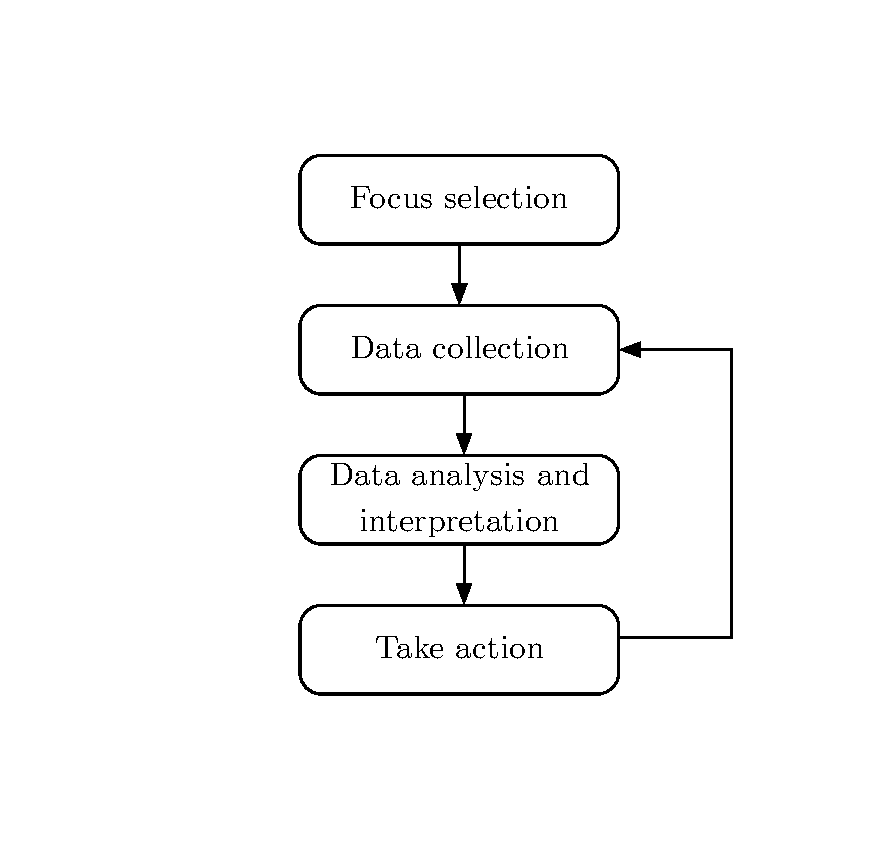
\includegraphics[width=0.3\linewidth]{figure/misc/ar.pdf}
\caption{Steps in action research}
\label{fig:action_research}
\end{figure}

AR is cyclical approach, meaning that the process does not have to be terminated after the fourth step. In this thesis work we started with selecting a focus and identifying a scope of visualization with one of stakeholders. then, we collected the first set of data from the Database and analyzed them. We took action by developing a prototype of automated visualization and presented it to the stakeholder in order to get some feedback for the improvement. Once we finalized the automated visualization, we began collecting the second set of data, by conducting semi-structured interview sessions with other stakeholders who use the Database as a tool in completing their daily assignments. During the interview sessions we recorded conversations. The second data analysis was done by transcribing the tape records, and the transcripts were analyzed using a scientific method for qualitative data analysis called \texttt{Coding} (will be described in Section~\ref{ME:coding}). In the final part of the work, the results from coding process were used for answering the research questions of this study.

\section{Data source}
Data used in this thesis work were collected from two main sources as follow:
\vspace{0.2em}
\begin{itemize}
    \item Raw JSON data from the Database
    \item Data from interviewing stakeholders
\end{itemize}
\vspace{0.2em}

\section{Data collection}
\subsection{Data from the Database}
To create an automated visualization, we extracted data from the Database. The best way that was suggested in retrieving data from the Database was to use an application program interface (API). At VCG, we were given a documentation that has a list of APIs and the description of how to use the APIs in order to get the data from the Database. In order to access the data, one has to be within the VCG network. Since we were not granted access, we did most of the work outside the company area and were forced to use the censored data file. The use of API is more dynamic than visualizing a static file. However, this does not make the step to retrieve data from the Database less meaningful, it is still the same data but later on, a static file will need to be replaced with a specific API to get the data from the Database.\\

The data found in the static file retrieved from the Database is in JSON format. A simple example of JSON object is shown in the  Listing~\ref{code:report_JSON_Object} below:

\begin{lstlisting}[caption=An example of JSON object, label=code:report_JSON_Object]
{
    "id": 1,
    "name": "Master Thesis report",
    "year": 2016,
    "place" : "Sweden",
    "examiner" : "Eric",
    "Supervisors": ["Truong", "Ulf", "Michel","Patrizio"]
}
\end{lstlisting}


\subsection{Data from interviewing stakeholders}
\label{ME:data_from_interviewing_stakeholders}
Three semi-structured interviews were conducted in the later part of the study after the automated visualization prototype was developed. The purpose of each interview was to collect needs from each stakeholder towards the automated visualization. We, as the interviewers developed a list of pre-determined questions aiming at answering the two research questions in Section~\ref{IN:rq} and their opinions on the automated visualization prototype.\\

The interview questions were divided into four groups based on the goal of each question, as follow:
\vspace{0.5em}
\begin{itemize}
    \item Getting to know interviewee,
    \item Emphasizing on understanding the use of the Database,
    \item Identifying the needs of stakeholders, and
    \item Opinions on the automated visualization prototype.
\end{itemize}
\vspace{0.5em}
During each interview session, an interviewee was asked many questions from the list in sequence, but he/she was not limited to those pre-determined questions. Some questions straying from the list were asked if the interviewers found it appropriated.\\

All conversions in the interviews were recorded which were then transcribed and analyzed later to answer the research questions. The list of questions and transcripts can be seen in Appendix~\ref{app2}.


\section{Data analysis}
\subsection{Meta-model from the JSON data}
To understand the raw JSON data from the Database, we created a meta-model of the data in order to see the schema of the file that specifies the relationship among the artifacts. The process of the meta-model was created is presented in Section~\ref{IM:analyzing_the_raw_json_data}.

\subsection{Coding}
\label{ME:coding}
Apart from the raw JSON data extracted from the Database, another set of data was collected from interviewing stakeholders. We started the analysis of the data by listening to the tape records twice in order to understand the conversations and to get some key points that the interviewee emphasized during the interviews. The process continued by transcribing the tape records word by word manually. We decided not to use any voice recognition software due to the fact that the software has to be trained for each voice, and it requires speakers to speak slowly making the interview inefficient.\\

The transcript files were then analyzed using coding method. To give a basic description what coding is, it is one of the methods used in qualitative data analysis especially the analysis of interview transcripts. It is the process of capturing essential words or phrases from set of data that give the same ideas, themes, and categories~\cite{OnlineQDA}. Before starting the coding process, a list of codes were created based on the goals of the pre-determined questions presented in Section~\ref{ME:data_from_interviewing_stakeholders}. Once we had the list of codes, each of us began coding the transcripts files. Then, we compared the results from coding together to summarize the coded data. The list of codes and the results are presented in Section~\ref{IM:coding_the_interview_transcripts} and Section~\ref{RE:results_from_the_coding}, respectively.


%%%%%
\begin{comment}
\subsection{Identifying stakeholders}
On referring to the article of Community Tool Box~\cite{community_tool_box}, there are three different kinds of stakeholders: primary stakeholders, secondary stakeholders and key stakeholders. In the later part of the study, we interviewed different stakeholders. Some of the advantages of interviewing the stakeholders include getting more ideas, obtaining different perspectives, helping to avoid misunderstanding of the problem, and also increasing the chances of delivering a valuable output to the stakeholders.\\

The primary stakeholders in our case are the people who are directly interacting with the Database, also named beneficiaries and we, the students are the target. The act of automated visualization can aid the beneficiaries in obtaining a simplified overview of a data found in the Database which in turn can provide a quick understanding of the needed artifacts and the interactions between these artifacts. \\

The secondary stakeholders are the ones who are indirectly affected by the Database. They are the ones who may be affected by the decision made by the stakeholders who interacts directly with the Database, which in turn will be due to the use of the obtained visualization. Our supervisors at the university can also be in a group of secondary stakeholders, they are not directly interacting with the obtained visualization but they also play a greater role in pushing forward our goals for delivering a good visualization. \\

The key stakeholders are the one funding this project and these can be the two supervisors from the company. All these stakeholders play a very important role in bringing efforts that could result to a better solution of the problem that we intend to resolve.\\

We, the students and as part of the primary stakeholders (targets), intended to provide a visualization output that could aid in quick understanding of the data stored in the Database and also provided the job opportunity for the need of having such a visualization tool to give the overview of the architecture. \\
\end{comment}